\documentclass[14pt]{article}
\usepackage[margin=1 in]{geometry}
\usepackage{amsmath}
\usepackage{graphicx}
\usepackage{listings}
\usepackage{algorithm}% http://ctan.org/pkg/algorithms
\usepackage{algpseudocode}% http://ctan.org/pkg/algorithmicx
\usepackage{hyperref}

\title{Chapter 2 Getting Started}
\author{Yue Chen}
\date{\today}

\begin{document}
\maketitle
Having $n = 2^k$, and $T(n) = n lg(n)$, we want to show that:

$$
T(2n) = 2n \cdot lg(2n)
$$
\begin{align*}
	T(2n) &= 2 * T(n) + 2n\\
	&= 2n \cdot lg(n) + 2n\\
	&= 2n \cdot (lg(n) + 1)\\
	&= 2n \cdot (lg(n) + lg(2))\\
	&= 2n \cdot lg(2n)\\
\end{align*}

\begin{algorithm}
\caption{Binary Search for 2.3-5}
\begin{algorithmic}[1]
\State $l \gets 0$
\State $r \gets A.length - 1$


\While{$l < r$}
	\State $i \gets \lfloor \frac{l + r}{2} \rfloor$
	\If {$A[i] = $target}
		\State \Return i
	\ElsIf {target $\geq A[i]$}
		\State $r \gets i - 1$
	\Else
		\State $l \gets i + 1$
	\EndIf
\EndWhile

\State \Return NIL

\end{algorithmic}
\end{algorithm}


\pagebreak

\section*{Exercise 2.3-7}
For me, this is a pretty intuitive way of thinking this question. It is too simple that I didn't believe it in the beginning and denied it after a few seconds of imagining the procedure in my head. However, I must admit that proving the correctness of this algorithm is non-trivial, at least for me.\\

I was taught by the solution written by Andrew Lohr in \url{https://sites.math.rutgers.edu/~ajl213/CLRS/Ch2.pdf}. Andrew really helped me a lot! Thanks!\\

Here I will just try to write my own understanding of the second part of this solution, where we try to do the two-way search.

In order to prevent too much copy-paste, let me put my own implementation of the algorithm written in Andrew's solution first.

\begin{figure}[h]
    \centering
    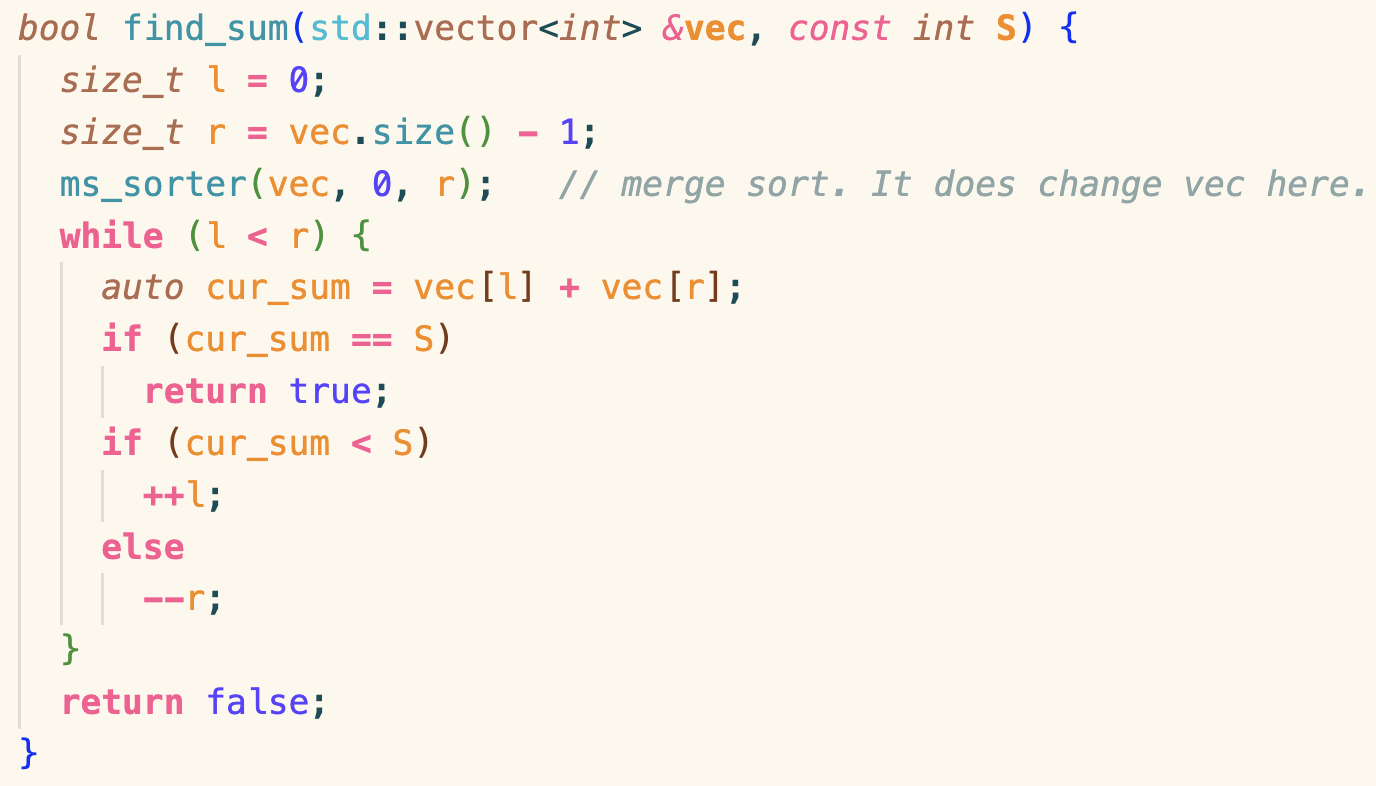
\includegraphics[width=4in]{img/find_sum.png}
\end{figure}

The essence of this algorithm is the second part --- the two-way search inside the while-loop. The most important thing to notice is that, as Andrew mentioned, if
$A[l] + A[r] < S$, we know that 
$\forall k \text{ such that } l \leq k \leq r, A[l] + A[k] < S$, and this works the other way. \\

 So, we know that the immediate next value/combination we should try is $A[l + 1] + A[r]$, assuming that the sequence is already sorted. This new combination gives us the next smallest sum we can try to approach the target $S$ gradually. And it works for the other side as well. \\
 
 Let me stop my innocent explanation here as Andrew has provided a rigorous proof of the correctness of this algorithm already. 



\pagebreak
\section*{Problems 2-2}
(a) We should also need to prove that all the elements in A still exist in the new sequence. \\

\noindent (b)\\

\textbf{Initialization}: 
Before the for-loop begins, we may have the smallest element of the sublist $A[i..j]$ to be somewhere between $i$ and $j$. Let's use $k$ to denote the index of the position of the index of the "smallest" element. So we must have $i \leq k \leq j$ since $j = A.length$ initially.\\

\textbf{Maintenance and Termination}: 
Now, we can see how it maintains the loop invariant merely by checking the situation when $j = k$ as other situations won't affect the result. 
When $j = k$, we have $A[j] = A[k]$ to be the smallest in the sublist $A[i..j]$. So it will swap the two elements $A[j]$ and $A[j - 1]$. Now we must have the smallest element to be in the sublist $A[i..j-1]$ in the current loop, which also gives us the property that the "smallest" one stays in $A[i..j']$ in the next loop, where $j' = j - 1$.\\

For the next and future loops, we will continue swapping the smallest element forward, resulting that the "smallest" one ends up to be in the position $i$.\\

\noindent (c)\\

\textbf{Initialization}:
Prior to the first iteration, we have $i = 1$ and the sublist $A[1..i-1]$ contains $i - 1 = 0$ elements so it is sorted.\\

\textbf{Maintenance}: 
Now, for every iteration, we would first have $i - 1$ sorted elements in the sublist $A[1..i-1]$.Then, since the inner for-loop gives us a termination that the smallest element in the sublist $A[i..A.length]$ will be swapped to the position $i$, we know that the $i^{th}$ smallest element is in the position $i$. Then we must have $A[1] \leq ... \leq A[i]$. \\

\textbf{Termination}: We would have $n$ sorted elements in the list $A[1..n]$\\

\noindent(d) Let $n = A.length$. For the inner loop, since we must go over all the iterations, it takes $n - i$ compares and swap (if required). Noting that swap takes constant time. And since we need to go through the outer loop from $i = 1$ to $i = n - 1$, the total cost is $\sum_{i = 1}^{n - 1} (n - i)$, which belongs to $\Theta (n^2)$. And since that all the iterations must be went over, the best case is also $\Theta(n^2)$.


\pagebreak
\section*{Problems 2-3}
(a) Assuming that multiplication and addition takes constant time. Then for every iteration, we would have $\Theta(1)$, resulting $T(n) = \Theta(n)$\\

\noindent(b)\\

\begin{algorithm}
\caption{naive polynomial-evaluation algorithm for 2-3}
\begin{algorithmic}
	\Statex $p \gets 0$
	\For{$k \gets 0, n$}
	\Statex $m \gets 1$
		\For{$i \gets 1, k$}\Comment{Calculate $x^k$}
			\State $m \gets m \cdot x$
		\EndFor
	\Statex $p \gets p + a_k \cdot m$
	\EndFor
\end{algorithmic}	
\end{algorithm}

Now that we need to calculate $x^k$ in every iteration, which requires $c_2k$ calculations. And since we iterate from $k = 0$ to $k = n$, in total we have $\Theta (n^2)$ complexity.\\

\noindent (c)\\


\textbf{Initialization}:
Before the loop begins, we have y = 0.\\

\textbf{Maintenance}:
$\forall 0 \leq i \leq n $, we can expand the expression of $y$ for each iteration as follows:
\begin{align}
	y &= a_i + x \cdot \sum_{k = 0}^{n-(i+1)} a_{k+i+1}x^k\\
	&= a_i + \sum_{k = 0}^{n-(i+1)} a_{k+i+1}x^{k+1}\\
	&= a_i + \sum_{k = 1}^{n-i} a_{k+i}x^{k}\\
	&= \sum_{k = 0}^{n-i} a_{k+i}x^{k}
\end{align}
In step 4, we recognize that $a_i$ is actually the term in the form $a_{k+i}x^k$ where k = 0.\\

\textbf{Termination}: 
And since in every iteration, $y$ is re-calculated without using previous $y$, we end up having $y$ to be the value calculated by the last iteration, where $i = 0$. It ends with the equation we want when $i = 0$.




\pagebreak
\section*{Problem 2-4}
(b)\\
The array that has $A[1] > .. > A[n]$ has the most inversions. It has $\sum_{i = 1}^{n-1}i$ pairs of inversion.\\

\noindent(c)\\
During the insertion sort procedure, we have a part where we would try to run a while-loop and insert the key in to the sorted part. Within that while-loop, we are actually operating/copying all pairs of inversion for that particular key. And inversion requires $i < j$ and $A[i] > A[j]$, it means that we only need to check the elements that has smaller index than the key. Summing the number of the operation we have made in the insertion sort for every key, we obtain the exact same number of total inversion.\\

\noindent(d)
My thoughts when designing this algorithm: \\
When we have two sublists, any element on the "right" side being copied to the merged list gives us that it has index greater than all the elements in the left sublist, and it has value smaller than all the elements in the left as well. Therefore, we may calculate the number of total inversions by summing up the length of the left sublist whenever the right-side element gets copied. 

\begin{algorithm}
\caption{Counting Inversion}
\begin{algorithmic}[1]
	\Statex MERGE(A, p, q, r)
	\State $n_1 := q - p + 1$
	\State $n_2 := r - q$
	\State let $L[1..n_1]$ and $R[1..n_2]$ be new arrays
	\For{$i := 1$ to $n_1$}
		\State $L[i] := A[p + i - 1]$
	\EndFor

	\For{$j := 1$ to $n_2$}
		\State $R[i] := A[q + j]$
	\EndFor
	
	\State $i := 1$
	\State $j := 1$
	\State $k := p$
	\State $c := 0$ \Comment{inversion count for this merge}
	\While{$i < n_1 + 1$ and $j < n_2 + 1$} 
		\If {$L[i] \leq R[j]$}
			\State $A[k] := L[i]$
			\State $i := i + 1$
		\Else
			\State $A[k] := R[j]$
			\State $j := j + 1$
			\State $c := c + (n_1 - i + 1)$
		\EndIf
		\State $k \gets k + 1$
	\EndWhile
	
	\State \Return c
\end{algorithmic}
\end{algorithm}

\pagebreak
\begin{algorithm}
\begin{algorithmic}[1]
	\Statex MERGESORT(A, p, r)
	\State $c \gets 0$
		\If{$ p < r $}
			\State $q \gets \lfloor \frac{p + r}{2} \rfloor$
			\State $c \gets c + $ MERGESORT(A, p, q)
			\State $c \gets c + $ MERGESORT(A, q+1, r)
			\State $c \gets c + $ MERGE(A, p, q, r)
			\State \Return c
		\EndIf
		\State \Return 0
	\State
	
\end{algorithmic}
\end{algorithm}

\pagebreak
























\end{document}